\subsubsection{2.3. Kết quả kiểm thử trên mô hình CNN + MGAT + FastKAN/MLP với toàn bộ phương thức}
\indent\indent Dưới đây là kết quả kiểm thử chi tiết của 12 mô hình CNN backbone + MGAT + FastKAN/MLP với toàn bộ phương thức, trong đó các giá trị được lấy từ lần chạy đạt kết quả cao nhất.\vspace{0.3cm}

%===================================================================
\textbf{* ResNet18 + MGAT + FastKAN/MLP:} 
\begin{table}[H] 
\centering 
\renewcommand{\arraystretch}{1.08} 
\caption{\centering Classification report của FastKAN(1) và MLP(2) trên toàn bộ phương thức với backbone ResNet18} 
\begin{tabular}{lccccccc} 
\hline \textbf{Lớp} & \textbf{P(1)} & \textbf{R(1)} & \textbf{F1(1)} & \textbf{P(2)} & \textbf{R(2)} & \textbf{F1(2)} & \textbf{Support} \\ \hline

cho-noi-cai-rang 
& 1.0000 & 0.9556 & \textbf{0.9773} 
& 0.9333 & 0.9333 & 0.9333 & 45 \\

dua-bo-bay-nui 
& 1.0000 & 1.0000 & \textbf{1.0000} 
& 0.9574 & 1.0000 & 0.9783 & 45 \\

hoi-lim 
& 0.9762 & 0.9111 & \textbf{0.9425} 
& 0.9130 & 0.9333 & 0.9231 & 45 \\

le-hoi-nghinh-ong 
& 0.9000 & 0.8000 & \textbf{0.8471} 
& 0.8261 & 0.8444 & 0.8352 & 45 \\

nghe-dan-tre 
& 1.0000 & 1.0000 & \textbf{1.0000} 
& 0.9565 & 0.9778 & 0.9670 & 45 \\

nghe-det-chieu 
& 0.9574 & 1.0000 & \textbf{0.9783} 
& 0.9348 & 0.9556 & 0.9451 & 45 \\

ok-om-bok 
& 0.9574 & 1.0000 & \textbf{0.9783} 
& 1.0000 & 0.8444 & 0.9157 & 45 \\

via-ba-chua-xu-nui-sam 
& 0.8235 & 0.9333 & \textbf{0.8750} 
& 0.8478 & 0.8667 & 0.8571 & 45 \\ 
\hline

\textbf{Accuracy} 
& & & \textbf{0.9500} 
& & & 0.9194 & 360 \\

\textbf{Macro avg} 
& \textbf{0.9518} & \textbf{0.9500} & \textbf{0.9498} 
& 0.9211 & 0.9194 & 0.9193 & 360 \\

\textbf{Weighted avg} 
& \textbf{0.9518} & \textbf{0.9500} & \textbf{0.9498} 
& 0.9211 & 0.9194 & 0.9193 & 360 \\ 
\hline 
\end{tabular} 
\end{table}

%===================================================================
\newpage
\textbf{* RegNetX400MF + MGAT + FastKAN/MLP:}
\begin{table}[H]
\centering
\renewcommand{\arraystretch}{1.08}
\caption{\centering Classification report của FastKAN(1) và MLP(2) trên toàn bộ phương thức với backbone RegNetX400MF}
\begin{tabular}{lccccccc}
\hline
\textbf{Lớp} &
\textbf{P(1)} & \textbf{R(1)} & \textbf{F1(1)} &
\textbf{P(2)} & \textbf{R(2)} & \textbf{F1(2)} &
\textbf{Support} \\
\hline

cho-noi-cai-rang
& 0.9778 & 0.9778 & \textbf{0.9778}
& 0.9565 & 0.9778 & 0.9670 & 45 \\

dua-bo-bay-nui
& 1.0000 & 1.0000 & \textbf{1.0000}
& 0.9375 & 1.0000 & 0.9677 & 45 \\

hoi-lim
& 0.8889 & 0.8889 & 0.8889
& 0.9318 & 0.9111 & \textbf{0.9213} & 45 \\

le-hoi-nghinh-ong
& 0.7727 & 0.7556 & 0.7640
& 0.8649 & 0.7111 & \textbf{0.7805} & 45 \\

nghe-dan-tre
& 1.0000 & 1.0000 & \textbf{1.0000}
& 0.9783 & 1.0000 & 0.9890 & 45 \\

nghe-det-chieu
& 0.9778 & 0.9778 & \textbf{0.9778}
& 1.0000 & 0.8889 & 0.9412 & 45 \\

ok-om-bok
& 0.9545 & 0.9333 & 0.9438
& 0.9556 & 0.9556 & \textbf{0.9556} & 45 \\

via-ba-chua-xu-nui-sam
& 0.7660 & 0.8000 & 0.7826
& 0.7593 & 0.9111 & \textbf{0.8283} & 45 \\
\hline

\textbf{Accuracy}
& & & 0.9167
& & & \textbf{0.9194} & 360 \\

\textbf{Macro avg}
& 0.9172 & 0.9167 & 0.9169
& \textbf{0.9230} & \textbf{0.9194} & \textbf{0.9188} & 360 \\

\textbf{Weighted avg}
& 0.9172 & 0.9167 & 0.9169
& \textbf{0.9230} & \textbf{0.9194} & \textbf{0.9188} & 360 \\
\hline
\end{tabular}
\end{table}
%===================================================================
\textbf{* MobileNetV3 Large + MGAT + FastKAN/MLP:}
\begin{table}[H]
\centering
\renewcommand{\arraystretch}{1.08}
\caption{\centering Classification report của FastKAN(1) và MLP(2) trên toàn bộ phương thức với backbone MobileNetV3 Large}
\label{tab:CRMobileNetV3LargeMGATFastKANMLP}
\begin{tabular}{lccccccc}
\hline
\textbf{Lớp} &
\textbf{P(1)} & \textbf{R(1)} & \textbf{F1(1)} &
\textbf{P(2)} & \textbf{R(2)} & \textbf{F1(2)} &
\textbf{Support} \\
\hline
cho-noi-cai-rang
& 0.9184 & 1.0000 & 0.9574
& 0.9778 & 0.9778 & \textbf{0.9778} & 45 \\

dua-bo-bay-nui
& 1.0000 & 1.0000 & \textbf{1.0000}
& 0.9783 & 1.0000 & 0.9890 & 45 \\

hoi-lim
& 0.9111 & 0.9111 & \textbf{0.9111}
& 0.8333 & 0.8889 & 0.8602 & 45 \\

le-hoi-nghinh-ong
& 0.8780 & 0.8000 & \textbf{0.8372}
& 0.8684 & 0.7333 & 0.7952 & 45 \\

nghe-dan-tre
& 1.0000 & 0.9778 & \textbf{0.9888}
& 0.9778 & 0.9778 & 0.9778 & 45 \\

nghe-det-chieu
& 0.9762 & 0.9111 & 0.9425
& 0.9767 & 0.9333 & \textbf{0.9545} & 45 \\

ok-om-bok
& 0.9773 & 0.9556 & \textbf{0.9663}
& 0.9130 & 0.9333 & 0.9231 & 45 \\

via-ba-chua-xu-nui-sam
& 0.8000 & 0.8889 & \textbf{0.8421}
& 0.7551 & 0.8222 & 0.7872 & 45 \\
\hline

\textbf{Accuracy}
& & & {\textbf{0.9306}}
& & & {0.9083} & 360 \\

\textbf{Macro avg}
& \textbf{0.9326} & \textbf{0.9306} & \textbf{0.9307}
& 0.9101 & 0.9083 & 0.9081 & 360 \\

\textbf{Weighted avg}
& \textbf{0.9326} & \textbf{0.9306} & \textbf{0.9307}
& 0.9101 & 0.9083 & 0.9081 & 360 \\
\hline
\end{tabular}
\end{table}
%===================================================================
\textbf{* MobileNetV3 Small + MGAT + FastKAN/MLP:}
\begin{table}[H]
\centering
\renewcommand{\arraystretch}{1.08}
\caption{\centering Classification report của FastKAN(1) và MLP(2) trên toàn bộ phương thức với backbone MobileNetV3 Small}
\begin{tabular}{lccccccc}
\hline
\textbf{Lớp} &
\textbf{P(1)} & \textbf{R(1)} & \textbf{F1(1)} &
\textbf{P(2)} & \textbf{R(2)} & \textbf{F1(2)} &
\textbf{Support} \\
\hline

cho-noi-cai-rang
& 0.9778 & 0.9778 & \textbf{0.9778}
& 0.8980 & 0.9778 & 0.9362 & 45 \\

dua-bo-bay-nui
& 1.0000 & 0.9778 & 0.9888
& 1.0000 & 1.0000 & \textbf{1.0000} & 45 \\

hoi-lim
& 0.9302 & 0.8889 & 0.9091
& 0.9111 & 0.9111 & \textbf{0.9111} & 45 \\

le-hoi-nghinh-ong
& 0.7857 & 0.7333 & 0.7586
& 0.8372 & 0.8000 & \textbf{0.8182} & 45 \\

nghe-dan-tre
& 0.9773 & 0.9556 & 0.9663
& 1.0000 & 0.9778 & \textbf{0.9888} & 45 \\

nghe-det-chieu
& 0.9130 & 0.9333 & 0.9231
& 0.9535 & 0.9111 & \textbf{0.9318} & 45 \\

ok-om-bok
& 0.9565 & 0.9778 & \textbf{0.9670}
& 0.9556 & 0.9556 & 0.9556 & 45 \\

via-ba-chua-xu-nui-sam
& 0.7600 & 0.8444 & 0.8000
& 0.8261 & 0.8444 & \textbf{0.8352} & 45 \\
\hline

\textbf{Accuracy}
& & & 0.9111
& & & \textbf{0.9222} & 360 \\

\textbf{Macro avg}
& 0.9126 & 0.9111 & 0.9113
& \textbf{0.9227} & \textbf{0.9222} & \textbf{0.9221} & 360 \\

\textbf{Weighted avg}
& 0.9126 & 0.9111 & 0.9113
& \textbf{0.9227} & \textbf{0.9222} & \textbf{0.9221} & 360 \\
\hline
\end{tabular}
\end{table}
%===================================================================
\textbf{* DenseNet121 + MGAT + FastKAN/MLP:}
\begin{table}[H]
\centering
\renewcommand{\arraystretch}{1.08}
\caption{\centering Classification report của FastKAN(1) và MLP(2) trên toàn bộ phương thức với backbone DenseNet121}
\begin{tabular}{lccccccc}
\hline
\textbf{Lớp} &
\textbf{P(1)} & \textbf{R(1)} & \textbf{F1(1)} &
\textbf{P(2)} & \textbf{R(2)} & \textbf{F1(2)} &
\textbf{Support} \\
\hline

cho-noi-cai-rang
& 1.0000 & 1.0000 & \textbf{1.0000}
& 0.9565 & 0.9778 & 0.9670 & 45 \\

dua-bo-bay-nui
& 1.0000 & 1.0000 & \textbf{1.0000}
& 1.0000 & 1.0000 & \textbf{1.0000} & 45 \\

hoi-lim
& 0.9302 & 0.8889 & 0.9091
& 0.9149 & 0.9556 & \textbf{0.9348} & 45 \\

le-hoi-nghinh-ong
& 0.8750 & 0.9333 & 0.9032
& 0.9111 & 0.9111 & \textbf{0.9111} & 45 \\

nghe-dan-tre
& 1.0000 & 0.9778 & 0.9888
& 0.9783 & 1.0000 & \textbf{0.9890} & 45 \\

nghe-det-chieu
& 0.9783 & 1.0000 & \textbf{0.9890}
& 1.0000 & 0.9556 & 0.9773 & 45 \\

ok-om-bok
& 0.9318 & 0.9111 & 0.9213
& 0.9333 & 0.9333 & \textbf{0.9333} & 45 \\

via-ba-chua-xu-nui-sam
& 0.9333 & 0.9333 & \textbf{0.9333}
& 0.9302 & 0.8889 & 0.9091 & 45 \\
\hline

\textbf{Accuracy}
& & & \textbf{0.9556}
& & & 0.9528 & 360 \\

\textbf{Macro avg}
& \textbf{0.9561} & \textbf{0.9556} & \textbf{0.9556}
& 0.9530 & 0.9528 & 0.9527 & 360 \\

\textbf{Weighted avg}
& \textbf{0.9561} & \textbf{0.9556} & \textbf{0.9556}
& 0.9530 & 0.9528 & 0.9527 & 360 \\
\hline
\end{tabular}
\end{table}

%===================================================================
\textbf{* ShuffleNetV2 1.0x + MGAT + FastKAN/MLP:}
\begin{table}[H]
\centering
\renewcommand{\arraystretch}{1.08}
\caption{\centering Classification report của FastKAN(1) và MLP(2) trên toàn bộ phương thức với backbone ShuffleNetV2 1.0x}
\begin{tabular}{lccccccc}
\hline
\textbf{Lớp} &
\textbf{P(1)} & \textbf{R(1)} & \textbf{F1(1)} &
\textbf{P(2)} & \textbf{R(2)} & \textbf{F1(2)} &
\textbf{Support} \\
\hline

cho-noi-cai-rang
& 1.0000 & 0.9111 & \textbf{0.9535}
& 0.9556 & 0.9556 & 0.9556 & 45 \\

dua-bo-bay-nui
& 0.9778 & 0.9778 & 0.9778
& 1.0000 & 0.9778 & \textbf{0.9888} & 45 \\

hoi-lim
& 0.8478 & 0.8667 & 0.8571
& 0.8958 & 0.9556 & \textbf{0.9247} & 45 \\

le-hoi-nghinh-ong
& 0.8333 & 0.8889 & \textbf{0.8602}
& 0.8750 & 0.7778 & 0.8235 & 45 \\

nghe-dan-tre
& 1.0000 & 0.9333 & 0.9655
& 0.9556 & 0.9556 & \textbf{0.9556} & 45 \\

nghe-det-chieu
& 0.8800 & 0.9778 & 0.9263
& 0.9565 & 0.9778 & \textbf{0.9670} & 45 \\

ok-om-bok
& 0.8667 & 0.8667 & 0.8667
& 1.0000 & 0.9333 & \textbf{0.9655} & 45 \\

via-ba-chua-xu-nui-sam
& 0.8837 & 0.8444 & \textbf{0.8636}
& 0.8200 & 0.9111 & 0.8632 & 45 \\
\hline

\textbf{Accuracy}
& & & 0.9083
& & & \textbf{0.9306} & 360 \\

\textbf{Macro avg}
& 0.9112 & 0.9083 & 0.9088
& \textbf{0.9323} & \textbf{0.9306} & \textbf{0.9305} & 360 \\

\textbf{Weighted avg}
& 0.9112 & 0.9083 & 0.9088
& \textbf{0.9323} & \textbf{0.9306} & \textbf{0.9305} & 360 \\
\hline
\end{tabular}
\end{table}

\indent Dựa trên kết quả kiểm thử chi tiết của các mô hình CNN backbone + MGAT + FastKAN/MLP trên tập dữ liệu kiểm thử với đầy đủ ba phương thức, tôi rút ra những nhận xét sau:\vspace{-0.1cm}
\begin{itemize}[label={--}, itemsep=1pt]
    \item \textbf{Hiệu quả vượt trội của đa phương thức:} So với mô hình CNN Baseline chỉ sử dụng hình ảnh (với F1-Score trung bình xấp xỉ 0.9), việc tích hợp thêm văn bản và âm thanh thông qua kiến trúc đồ thị (MGAT) đã giúp cải thiện đáng kể độ chính xác ở hầu hết các backbone. Đặc biệt, sự cải thiện thể hiện rõ rệt nhất ở các lớp có độ nhập nhằng cao về mặt thị giác như \textit{le-hoi-nghinh-ong} và \textit{via-ba-chua-xu-nui-sam}.
    \item \textbf{So sánh FastKAN và MLP trên từng kiến trúc:}\vspace{-0.1cm}
    \begin{itemize}[label={+}, itemsep=1pt]
        \item Với ResNet18: Bộ phân lớp FastKAN thể hiện sự vượt trội hơn hẳn MLp. Cụ thể, ResNet18 + FastKAN đạt độ chính xác lên tới 0.95, vượt xa kết quả của MLP (0.9194). Đáng chú ý, tại lớp \textit{via-ba-chua-xu-nui-sam} vốn rất khó phân loại, FastKAN giúp tăng Recall từ 0.86 (MLP) lên 0.93, chứng tỏ khả năng học các biên quyết định phi tuyến phức tạp tốt hơn hẳn so với cấu trúc truyền thống của MLP.
        \item Với DenseNet121: Đây là kiến trúc cho kết quả cao nhất trong tất cả các thử nghiệm, với độ chính xác đạt trên 0.95 ở cả hai biến thể FastKAN và MLP. Kết quả này ghi nhận mức cải thiện khoảng 5\% so với mô hình CNN Baseline đơn phương thức.
        \item Với MobileNetV3 Large: FastKAN tiếp tục khẳng định ưu thế với Accuracy 0.9306 (so với 0.9083 của MLP). Mô hình này đạt điểm tuyệt đối (1.0) ở lớp \textit{dua-bo-bay-nui} và cải thiện đáng kể F1-Score cho lớp \textit{le-hoi-nghinh-ong} (0.8372 so với 0.7952), cho thấy sự kết hợp giữa một backbone nhẹ và một classifier mạnh mẽ là hướng đi đầy tiềm năng.
        \item Với các backbone MobileNetV3 Small, ShuffleNetV2, RegNet: Kết quả cho thấy MLP lại hoạt động hiệu quả hơn hoặc tương đương FastKAN. Ví dụ, với ShuffleNetV2 1.0x, MLP đạt 0.9306 trong khi FastKAN chỉ đạt 0.9083. Điều này có thể lý giải rằng khi đặc trưng đầu vào từ backbone bị nén quá mức (lượng thông tin thưa thớt), sự phức tạp của FastKAN có thể dẫn đến hiện tượng overfitting nhẹ, trong khi cấu trúc đơn giản của MLP lại giúp mô hình tổng quát hóa tốt hơn.
    \end{itemize}
\end{itemize}


%===================================================================
Dưới đây là bảng tổng hợp và biểu đồ thể hiện kết quả trung bình của tất cả 12 mô hình CNN backbone + MGAT + FastKAN/MLP:
\begin{table}[H]
\centering
\renewcommand{\arraystretch}{1.2}
\setlength{\tabcolsep}{6pt}
\caption{\centering Kết quả kiểm thử trung bình của tất cả các mô hình CNN backbone + MGAT + FastKAN/MLP trên toàn bộ phương thức}
\begin{tabular}{llcccc}
\hline
\textbf{Backbone Model (+ MGAT)} & \textbf{Classifier} & \textbf{Accuracy} & \textbf{Precision} & \textbf{Recall} & \textbf{F1-Score} \\ 
\hline

% ResNet18
\multirow{2}{*}{ResNet18} 
& FastKAN & \textbf{0.9343} & \textbf{0.9358} & \textbf{0.9343} & \textbf{0.9341} \\
& MLP & 0.9000 & 0.9030 & 0.9000 & 0.8996 \\ 
\hline

% RegNetX400MF
\multirow{2}{*}{RegNetX400MF} 
& FastKAN & 0.9074 & 0.9094 & 0.9074 & 0.9071 \\
& MLP & \textbf{0.9092} & \textbf{0.9134} & \textbf{0.9092} & \textbf{0.9090} \\ 
\hline

% MobileNetV3 Large
\multirow{2}{*}{MobileNetV3 Large} 
& FastKAN & \textbf{0.9260} & \textbf{0.9283} & \textbf{0.9260} & \textbf{0.9258} \\
& MLP & 0.9056 & 0.9059 & 0.9056 & 0.9043 \\ 
\hline

% MobileNetV3 Small
\multirow{2}{*}{MobileNetV3 Small} 
& FastKAN & 0.9055 & 0.9111 & 0.9055 & 0.9041 \\
& MLP & \textbf{0.9120} & \textbf{0.9174} & \textbf{0.9120} & \textbf{0.9118} \\ 
\hline

% DenseNet121
\multirow{2}{*}{DenseNet121} 
& FastKAN & \textbf{0.9435} & \textbf{0.9477} & \textbf{0.9435} & \textbf{0.9438} \\
& MLP & 0.9417 & 0.9455 & 0.9417 & 0.9413 \\ 
\hline

% ShuffleNetV2
\multirow{2}{*}{ShuffleNetV2 1.0x} 
& FastKAN & 0.8981 & 0.9007 & 0.8981 & 0.8980 \\
& MLP & \textbf{0.9204} & \textbf{0.9236} & \textbf{0.9204} & \textbf{0.9203} \\ 
\hline

\end{tabular}
\label{tab:avg_performance_comparison}
\end{table}

\begin{figure}[H]
    \centering
    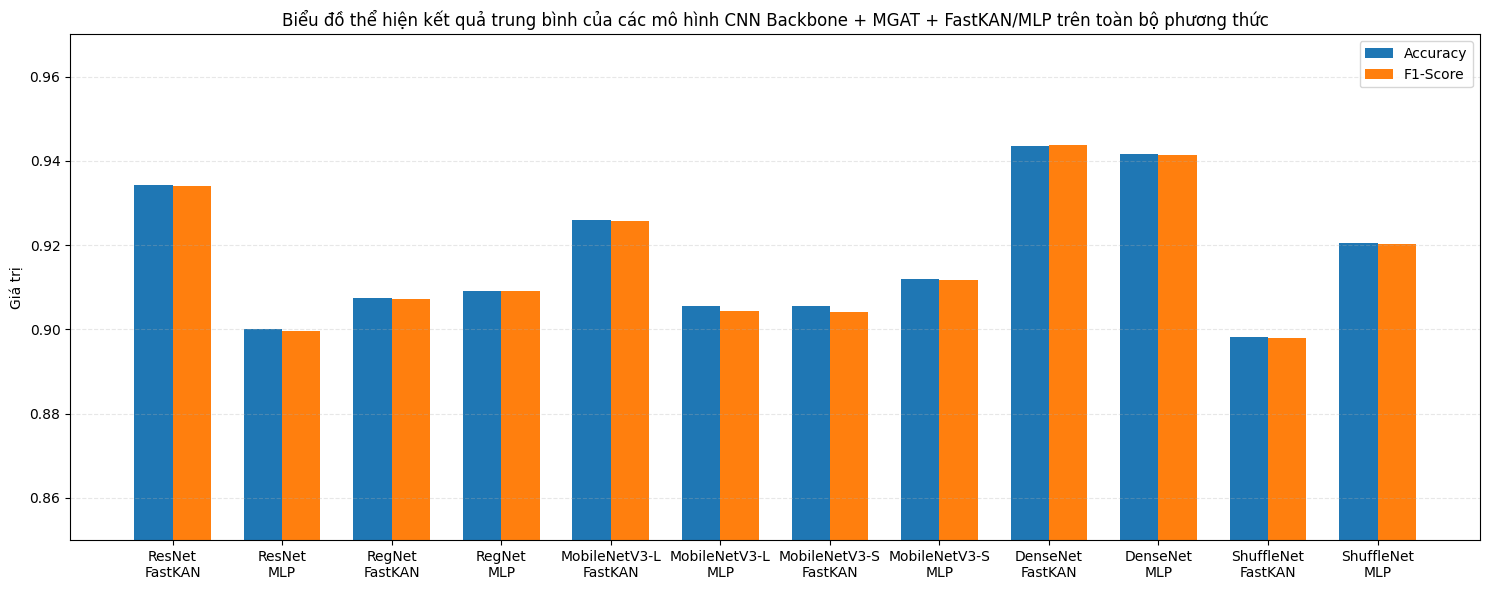
\includegraphics[width=\linewidth]{images/part-02/chap-03/sec-02/PipelineFull.png}
    \caption{\centering Biểu đồ thể hiện kết quả kiểm thử trung bình của tất cả các mô hình CNN backbone + MGAT + FastKAN/MLP trên toàn bộ phương thức}
    \label{fig:KQPipelineFull}
\end{figure}

\indent Dựa trên bảng tổng hợp và biểu đồ thể hiện kết quả trung bình của 12 mô hình trên toàn bộ phương thức, tôi đưa ra các kết luận sau:\vspace{-0.1cm}
\begin{itemize}[label={--}, itemsep=1pt]
    \item \textbf{Khẳng định tính hiệu quả của phương pháp đề xuất:} Hầu hết các mô hình MGAT (dù kết hợp với FastKAN hay MLP) đều vượt qua ngưỡng hiệu năng của CNN Baseline (cao nhất ~0.90). Nổi bật nhất là sự kết hợp DenseNet121 + MGAT + FastKAN đạt tới \textbf{0.9435} và ResNet18 + MGAT + FastKAN đạt \textbf{0.9343}. Điều này chứng minh rằng việc mô hình hóa dữ liệu dưới dạng đồ thị đa phương thức đã thành công trong việc tận dụng thông tin bổ trợ từ văn bản và âm thanh để bù đắp các khoảng trống tri thức mà mô hình đơn phương thức bỏ sót.
    \item \textbf{Sự tương quan giữa FastKAN và MLP:} Kết quả kiểm thử chỉ ra không có một bộ phân lớp nào là tối ưu cho mọi trường hợp:
    \begin{itemize}[label={+}, itemsep=1pt]
        \item \textbf{FastKAN} là lựa chọn tối ưu cho các mô hình có khả năng trích xuất đặc trưng mạnh (backbone lớn/sâu như ResNet, DenseNet, MobileNet Large). Khả năng biểu diễn hàm linh hoạt của KAN giúp khai thác triệt để lượng thông tin phong phú từ các backbone, điều này đã giúp đẩy độ chính xác phân lớp lên mức cao hơn.
        \item \textbf{MLP} lại là giải pháp an toàn và hiệu quả cho các mô hình gọn nhẹ (backbone nhỏ như MobileNet Small, ShuffleNet). Trong trường hợp tài nguyên tính toán cực kỳ hạn chế, sự kết hợp ShuffleNetV2 + MLP (0.9204) mang lại kết quả rất ấn tượng.
    \end{itemize}
\end{itemize}